\section{Mean Field Theory}\TODO{reference: D. Tong - statistical field theory, 1 | D. Tong - statistical physics, 5}

Mean field theory is a powerful approximation method used to study phase transitions and critical phenomena in many-body systems. The basic idea behind mean field theory is to replace the complex interactions between particles in the system with an average or ``mean'' field that each particle experiences. This simplification allows us to derive self-consistent equations for the order parameter and analyze the behavior of the system near the critical point.

Let us concentrate on a classical model, the Ising model, which is a prototypical model for studying ferromagnetic phase transitions.

\subsection{Ising Model} \TODO{insert images of spins on a lattice}

The Ising model consists of a lattice of spins, where each spin \(s_i\) can take on values of +1 or -1. The Hamiltonian of the Ising model is given by:
\[
    H = - J \sum_{\langle i,j \rangle} s_i s_j - h \sum_i s_i,
\]
where \(J\) is the coupling constant that determines the strength of the interaction between neighboring spins, \(h\) is the external magnetic field, and the sum \(\langle i,j \rangle\) runs over pairs of \textbf{nearest-neighbor} spins. The first term in the Hamiltonian represents the interaction between neighboring spins, which favors alignment (ferromagnetic order) when \(J > 0\). The second term represents the coupling of the spins to the external magnetic field, which tends to align the spins in the direction of the field.

\begin{definition}[Coordination Number]
    The coordination number \(z\) of a lattice is the number of nearest neighbors that each site has. For example, in a two-dimensional square lattice, each site has 4 nearest neighbors, so the coordination number is \(z = 4\). In a three-dimensional cubic lattice, each site has 6 nearest neighbors, so the coordination number is \(z = 6\). The coordination number plays an important role in determining the behavior of the system and the nature of the phase transition.
\end{definition}

Our aim is to study the equilibrium properties (where observables can effectively be calculated through thermal averaging) of the Ising model and understand the nature of the phase transition it exhibits. To do this, we will apply mean field theory to derive self-consistent equations for the magnetization (order parameter) and analyze the behavior of the system near the critical point.

Each configuration of the system is specified by the set of spin values \(\{s_i\}_{i=1}^N\), and it is associated to a probability given by the Boltzmann distribution:
\[
    P(\{s_i\}) = \frac{1}{\mathcal{Z}} e^{-\beta H(\{s_i\})},
\]
where \(\mathcal{Z}\) is the \textbf{partition function}, defined as the sum over all possible configurations:
\[
    \mathcal{Z} = \sum_{\{s_i\}} e^{-\beta H(\{s_i\})}.
\]

\begin{example}[Pair of spins]
    When we have only two spins, the partition function can be calculated explicitly. The Hamiltonian for two spins \(s_1\) and \(s_2\) is given by:
    \[
        H = - J s_1 s_2 - h (s_1 + s_2),
    \]
    where the sum is removed since we only have two spins. We can now compute the energy for each of the four possible configurations of the spins:
    \begin{itemize}
        \item \(s_1 = +1,\, s_2 = +1\): \(H = - J - 2h\).
        \item \(s_1 = +1,\, s_2 = -1\): \(H = J\).
        \item \(s_1 = -1,\, s_2 = +1\): \(H = J\).
        \item \(s_1 = -1,\, s_2 = -1\): \(H = - J + 2h\).
    \end{itemize}
    The partition function is then given by:
    \[
        \mathcal{Z} = e^{\beta J + 2\beta h} + 2 e^{-\beta J} + e^{\beta J - 2\beta h}.
    \]

    If we now wanted to compute the probability of finding the system in the configuration \(s_1 = +1,\, s_2 = +1\), we would use the Boltzmann distribution:
    \[
        P(s_1 = +1,\, s_2 = +1) = \frac{e^{\beta J + 2\beta h}}{\mathcal{Z}}.
    \]

    For the magnetization, we can compute the average spin per site:
    \[
        M = \left\langle \sum_{i} s_i \right\rangle_c, \quad m = \frac{M}{N} = \frac{1}{N} \left\langle s_1 + s_2 \right\rangle_c,
    \]
    where the summations run over the configuration space.
    \[
        m = \sum_{\langle s_i \rangle} p(\{s_i\}) \left( \frac{1}{N} \sum_{i} s_i \right),
    \]
    where the sum runs over all possible configurations of the spins. In this case, we can explicitly compute the magnetization by summing over the four configurations.
\end{example}

If we were now to consider a system with \(N=100\), we would have \(2^{100}\) possible configurations for a chain with \(z=2\), which is an astronomically large number. This makes it impossible to compute the partition function and the magnetization by explicitly summing over all configurations. This is where mean field theory comes into play, as it allows us to approximate the behavior of the system without needing to consider every possible configuration.

\subsection{Mean Field Approach - Euristic}

Let us now apply the mean field approximation to the Ising model. The key idea is to replace the interaction term in the Hamiltonian with an average or ``mean'' field that each spin experiences. This allows us to derive a self-consistent equation for the magnetization.

It is a \textit{euristic} approach, which is not exact but provides a good approximation, remaining not systematic, not rigorous and hard to fully justify. We will see how it can be derived from a more rigorous approach, which is the \textbf{Landau-Ginzburg effective field theory}.

There are many versions of this approach (different implementations of the approximation), but the idea is almost the same: we want to replace some microscopic degrees of freedom with an average field, which is the mean field. The mean field is defined as the average value of the spin at a given site:

Let us rewrite the Hamiltonian of the Ising model
\[
    H = - J \sum_{\langle s_i, s_j \rangle} s_i s_j - h \sum_i s_i.
\]
If we now consider the case in which the coupling constant \(J\) is positive (\(J>0\) which corresponds to a ferromagnetic interaction), and a null external magnetic field (\(h=0\)), the Hamiltonian simplifies to:
\[
    H = - J \sum_{\langle s_i, s_j \rangle} s_i s_j.
\]
In this case the system exhibits a phase transition at a critical temperature \(T_c\), below which the spins tend to align and the system enters an ordered ferromagnetic phase, while above \(T_c\) the spins are disordered and the system is in a paramagnetic phase.

Being interested in the behavior of the magnetization, we can express it as a thermal average in the canonical ensemble:
\[
    \left\langle \frac{1}{N} \sum_{i} s_i \right\rangle_c = \frac{1}{N} \sum_{\{s_i\}} \left( \sum_{i} s_i \right) \frac{e^{-\beta H(\{s_i\})}}{\mathcal{Z}},
\]
where the sum runs over all possible configurations of the spins. The mean field approximation consists in building a term which encodes the average effect of the neighboring spins on a given spin: it is natural to think about building this average field from the magnetization, so let us analyze it in more detail. The magnetization can assume the following values:
\[
    M \in \left[ -N,\, -N+2,\, -N+4,\, \ldots,\, +N \right],
\]
where the values change by 2 because each spin can flip from +1 to -1 or vice versa. The magnetization per site is then given by:
\[
    m = \frac{M}{N} \in \left[ -1,\, -1 + \frac{2}{N},\, -1 + \frac{4}{N},\, \ldots,\, +1 \right].
\]

The average field we are building has to be proportional to the magnetization \(m\), which serves as a measure of the degree of order in the system. Thus we can express the sum over configurations of the spins as a sum over the magnetization \(M\) and then a sum over all configurations that correspond to that magnetization:
\[
    \sum_{\{s_i\}_{i=1}^N} [\dots] = \sum_{M=-N}^{N} \sum_{\{s_i\}_{i=1}^N} \delta\left(\sum_{i} s_i - M\right)[\dots],
\]
where we have introduced a delta function to enforce the constraint that the sum of the spins equals the magnetization \(M\). This allows us to rewrite the partition function as a sum over the magnetization, but let's understand better the meaning of this delta function through an example.

\begin{example}[\(N=2\)]
    If we have only two spins, the possible configurations and their corresponding magnetizations are:
    \begin{itemize}
        \item A: \(s_1 = +1,\, s_2 = +1\): \(M = 2\).
        \item B: \(s_1 = +1,\, s_2 = -1\): \(M = 0\).
        \item C: \(s_1 = -1,\, s_2 = +1\): \(M = 0\).
        \item D: \(s_1 = -1,\, s_2 = -1\): \(M = -2\).
    \end{itemize}
    The delta function \(\delta\left(\sum_{i} s_i - M\right)\) ensures that we only sum over configurations that correspond to a specific magnetization \(M\).

    Let us analyze the contribution of each configuration to the partition function: starting from a sum over all configurations, we get
    \[
        \mathcal{Z} = \sum_{\{s_i\}} e^{-\beta H(\{s_i\})} = e^{- \beta H(A)} + e^{-\beta H(B)} + e^{-\beta H(C)} + e^{-\beta H(D)},
    \]
    where \(H(A)\), \(H(B)\), \(H(C)\), and \(H(D)\) are the Hamiltonian evaluated at each configuration: considering the case \(h=0\) for simplicity, we have
    \[
        H(A) = -J, \quad H(B) = J, \quad H(C) = J, \quad H(D) = -J.
    \]
    Thus the partition function can be rewritten as
    \[
        \mathcal{Z} = 2 (e^{\beta J} + e^{-\beta J}).
    \]

    We now want to get the same result using the sum over magnetization, which is given by
    \[
        \mathcal{Z} = \sum_{M = -2}^2 \sum_{\{s_i\}} \delta\left(\sum_{i} s_i - M\right) e^{-\beta H(\{s_i\})} = \sum_{M = -2}^2 e^{-\beta H(M)} \sum_{\{s_i\}} \delta\left(\sum_{i} s_i - M\right) = 2 (e^{\beta J} + e^{-\beta J}),
    \]
    where we have used the fact that the Hamiltonian depends only on the magnetization \(M\) and not on the specific configuration of the spins, and that the sum over configurations for each magnetization value is just the number of configurations with that value of magnetization. This example illustrates how the sum over configurations can be rewritten as a sum over magnetization, with the delta function ensuring that we only consider configurations that correspond to a specific magnetization.
\end{example}

Now we can implement the mean field approximation by replacing the interaction term in the Hamiltonian with an average field that each spin experiences. This average field is proportional to the magnetization \(m\), which serves as a measure of the degree of order in the system: in a fixed magnetization sector (\(m\)-sector) we can replace the interaction term with an effective field that depends on the magnetization (reinserting the external magnetic field \(h\)):
\[
    H_{mf} (\{s_i\}, m) = -J \sum_{\langle i, j \rangle} s_i \, m - h \sum_i s_i,
\]
where we are summing over single sites (only \(s_i\) appears in the sum), but we kept the notation of the sum over nearest neighbors to indicate that the effective field is proportional to the number of nearest neighbors (coordination number \(z\)) and the magnetization \(m\). This substitution corresponds to the intuition that each spins feels an average magnetization from the surrounding neighbors, and the crucial point is that now the spin variable enters linearly in the effective Hamiltonian. This is the point where we have to accept that this method works even if it is hard to justify: there exist some ad-hoc argument, but it would be meaningless to use those since we will anyway present the Landau-Ginzburg effective field theory in the following sections, which then will make us able to justify this approximation in a systematic way.

\begin{remark}
    The hamiltonian \(H_{mf}\) is independent of the specific configuration of the spins \(\{s_i\}\), as long as
    \[
        \sum_{i} s_i = M,
    \]
    So that we have efficiently replaced the interaction term with an average field that depends only on the magnetization \(m\). This allows us to derive a self-consistent equation for the magnetization and analyze the behavior of the system near the critical point without needing to consider every possible configuration of the spins.
\end{remark}

If we continue the computation of the mean field hamiltonian  we get
\[
    H_{mf} (\{s_i\}, m) = -J m \sum_{\langle i, j \rangle} s_i - h \sum_i s_i = - (J \frac{z}{2} m + h) \sum_i s_i = - (\frac{J z m}{2} + h) Nm,
\]
where we have used the fact that the sum over the spins is equal to the magnetization \(M = Nm\) and the sum over the nearest neighbors gives a factor of the coordination number \(\frac{Nz}{2}\).\footnote{When we count the same site for each of its n.n., we are counting each \(s_i\) a number of \(z\) times, but we have to divide by 2 to avoid double-counting. Thus the total is \(N\cdot \frac{z}{2}\).} This mean field Hamiltonian describes a system of non-interacting spins in an \textit{effective magnetic field} that depends on the magnetization \(m\) and the external field \(h\).

The average magnetization per spin in the canonical ensamble can now be performed easily applying the mean field approximation:
\[
    \begin{aligned}
        \left\langle \frac{1}{N} \sum_{i} s_i \right\rangle_c & = \sum_{m \in [-1, \ldots, +1]} m \sum_{\{s_i\}} \delta\left(\sum_{i} s_i - Nm\right) \frac{e^{-\beta H_{mf}(m)}}{\mathcal{Z}} \\
                                                              & = \frac{1}{\mathcal{Z}} \sum_{m} m e^{-\beta H_{mf}(m)} \left[ \sum_{\{s_i\}} \delta\left(\sum_{i} s_i - Nm\right) \right],    \\
    \end{aligned}
\]
where the last term identifies a sum over all the configurations of the spins that correspond to a given magnetization \(m\). Note that a configuration of \(N_{\uparrow}\) of up spins and \(N_{\downarrow}\) of down spins corresponds to a magnetization
\[
    m = \frac{N_{\uparrow} - N_{\downarrow}}{N} = \frac{2 N_{\uparrow} - N}{N} = 2 \frac{N_{\uparrow}}{N} - 1.
\]
The number of such configurations is given by the binomial coefficient:
\[
    \binom{N}{N_{\uparrow}} = \frac{N!}{N_{\uparrow}! (N - N_{\uparrow})!} = \Omega(N_\uparrow),
\]
which we can approximate using Stirling's formula for large \(N\):
\[
    \log(\Omega(N_\uparrow)) \approx N \log N - N_{\uparrow} \log N_{\uparrow} - (N - N_{\uparrow}) \log (N - N_{\uparrow}),
\]
which after some algebraic manipulations can be rewritten as
\[
    \log(\Omega(N_\uparrow)) \approx N \left[ \log(2) - \frac{(1+m)}{2}\log (1+m) - \frac{(1-m)}{2}\log (1-m) \right].
\]
Thus we have found an expression for the number of configurations that correspond to a given magnetization \(m\), which can be used to compute the final form of the magnetization:
\[
    \left\langle \frac{1}{N} \sum_{i} s_i \right\rangle_c = \frac{1}{\mathcal{Z}} \sum_{m} m e^{-\beta H_{mf}(m)} \Omega(m) = \frac{1}{\mathcal{Z}} \sum_{m} m e^{-\beta N f(m)},
\]
where we have defined the function \(f(m)\) as
\[
    f(m) = - hm - \frac{Jzm^2}{2} - \frac{1}{\beta} \left[ \log(2) - \frac{(1+m)}{2}\log (1+m) - \frac{(1-m)}{2}\log (1-m) \right],
\]
which can be interpreted as a \textbf{free energy density} (per site) that depends on the magnetization \(m\). Indeed we have the last sum over the magnetization \(m\) getting dominated by the minimum of the function \(f(m)\) in the thermodynamic limit \(N \to \infty\), while the other terms get suppressed by the factor \(e^{-\beta N f(m)}\).\footnote{Since we always have to consider an enormously large \(N\) (the real world is at the thermodynamic limit), even small variations in \(f(m)\) will be exponentially suppressed.} Thus the average magnetization can be approximated as
\[
    \left\langle \frac{1}{N} \sum_{i} s_i \right\rangle_c \approx \frac{1}{e^{-\beta N f(m^*)}} \left( m^* e^{-\beta N f(m^*)} \right) = m^*, \qquad \frac{\partial f(m)}{\partial m}\bigg|_{m^*} = 0,
\]
where \(m^*\) is the value of \(m\) that minimizes the function \(f(m)\).\TODO{Add a figure of a parabula with the minimum at m-star.} This is known as a \textbf{saddle point approximation}, which is a common technique used in statistical mechanics to evaluate integrals or sums that are dominated by the contribution of a single point (the minimum of the free energy in this case). We have used the same approximation to compute the partition function \(\mathcal{Z}\) in the denominator as well, which is given by
\[
    \mathcal{Z} = \sum_{m} e^{-\beta N f(m)} \approx e^{-\beta N f(m^*)}.
\]

\paragraph{Self-consistency relation.}
Now computing the derivative of \(f(m)\) with respect to \(m\) and setting it to zero, we get the self-consistent equation for the magnetization:
\[
    \beta(h + J z m) = \frac{1}{2} \log\left( \frac{1+m}{1-m} \right) = \tanh^{-1}(m),
\]
where the last step is obtained after algebraic manipulations. This equation can be rewritten as
\[
    m = \tanh\left( \beta h_{eff} \right), \quad h_{eff} = h + J z m,
\]
where \(h_{eff}\) is the effective magnetic field that each spin experiences due to the mean field approximation. This self-consistent equation can be solved numerically to find the magnetization \(m\) as a function of temperature \(T\) and external field \(h\), allowing us to analyze the behavior of the system near the critical point and understand the nature of the phase transition. The effective field \(h_{eff}\) captures the influence of the neighboring spins on a given spin, and the self-consistent equation reflects the fact that the magnetization \(m\) depends on itself through the effective field. This is a hallmark of mean field theory, where the order parameter (magnetization) is determined by a self-consistent equation that takes into account the average effect of the interactions in the system.


\section{Self-Consistency and Phase Transitions}

In order to solve the self-consistent equation, we can analyze it graphically by plotting the function \(m\) on the left-hand side and the function \(\tanh\left( \beta h_{eff} \right)\) on the right-hand side as functions of \(m\). The points where these two functions intersect correspond to the solutions of the self-consistent equation. By varying the temperature \(T\) and the external field \(h\), we can observe how the number and nature of the solutions change, which provides insights into the phase transition and critical behavior of the system. Let us start from the case \(h=0\):\TODO{fix the plot}
\begin{figure}[H]
    \begin{minipage}{0.6\textwidth}
        \centering
        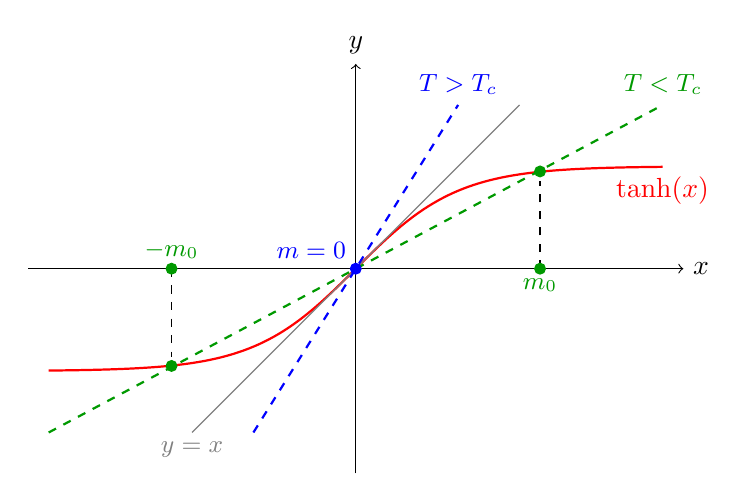
\begin{tikzpicture}[scale=1.3]

            \draw[->] (-3.2,0) -- (3.2,0) node[right] {$x$};
            \draw[->] (0,-2) -- (0,2) node[above] {$y$};

            \draw[thick,red,domain=-3:3,samples=200]
            plot (\x,{tanh(\x)}) node[below] {$\tanh(x)$};

            \draw[gray] (1.6,1.6) -- (-1.6,-1.6)
            node[below] {\small $y=x$};

            \draw[blue,thick,dashed] (-1,-1.6) -- (1,1.6)
            node[above] {\small $T>T_c$};

            \draw[green!60!black,thick,dashed] (-3,-1.6) -- (3,1.6)
            node[above] {\small $T<T_c$};

            \draw[dashed] (1.8,0) -- (1.8,0.859);
            \draw[dashed] (-1.8,0) -- (-1.8,-0.859);

            \filldraw[green!60!black] (1.8,0) circle (1.5pt) node[below] {\small $m_0$};
            \filldraw[green!60!black] (-1.8,-0) circle (1.5pt) node[above] {\small $-m_0$};
            \filldraw[green!60!black] (1.8,0.95) circle (1.5pt);
            \filldraw[green!60!black] (-1.8,-0.95) circle (1.5pt);

            \filldraw[blue] (0,0) circle (1.5pt) node[above left] {\small $m=0$};
        \end{tikzpicture}
    \end{minipage}
    \hfill
    \begin{minipage}{0.35\textwidth}
        The graphical solution shows that for \(T > T_c\) the only intersection is at the origin, yielding \(m=0\): this corresponds to the \textbf{paramagnetic phase}. For \(T < T_c\), instead, the line intersects the curve at two symmetric non-zero points, corresponding to two stable ordered states with opposite magnetization: this is the \textbf{ferromagnetic phase}.
    \end{minipage}
\end{figure}
\begin{itemize}
    \item For \(T > T_c\), there is only one solution at \(m = 0\), which corresponds to the paramagnetic phase where the spins are disordered and there is no net magnetization.
    \item For \(T < T_c\), there are three solutions: one at \(m = 0\) and two symmetric solutions at \(m = \pm m^*\), which correspond to the ferromagnetic phase where the spins are aligned and there is a non-zero magnetization. The solution at \(m = 0\) becomes unstable (not a minimum) in this regime, while the two symmetric solutions represent the stable ordered phases.
    \item At \(T = T_c\), the solution at \(m = 0\) becomes marginally stable, and the system undergoes a second-order phase transition from the paramagnetic phase to the ferromagnetic phase. The magnetization \(m\) changes continuously across the transition, and there is no latent heat associated with the transition.
\end{itemize}
The critical temperature \(T_c\) is determined by the condition that the slope of the \(\tanh\) function at \(m = 0\) equals 1, which gives
\[
    \beta_c J z = 1 \quad \Rightarrow \quad T_c = \frac{J z}{k_B},
\]
where \(k_B\) is the Boltzmann constant.

We can now study the beaviour of the magnetization as a function of temperature.\TODO{add plot of m vs T}
As we decreas the temperature \(T\) below \(T_c\), the magnetization \(m\) increases continuously from zero, indicating the onset of ferromagnetic order. We got two symmetric solutions for the magnetization, which correspond to the two possible orientations of the spins in the ferromagnetic phase. The magnetization \(m\) serves as an order parameter that characterizes the phase transition: it is zero in the paramagnetic phase and becomes non-zero in the ferromagnetic phase, indicating the spontaneous breaking of symmetry.

We can obtain the plot of the free energy as a function of the magnetization \(m\) for different temperatures to visualize the phase transition. This can be done numerically by studying the expression for the free energy density \(f(m)\) close to the critical temperature \(T_c\), i.e. expanding it in a power series around \(m = 0\) to analyze the behavior near the critical point:
\[
    \begin{aligned}
        f(m) & = Jz \left[\frac{m^2}{2} - \frac{1}{\beta J z}\left( \frac{(\beta h_{eff})^2}{2} - \frac{(\beta h_{eff})^4}{12} \right)\right] - \frac{\log 2}{\beta} \\
             & = \frac{Jz}{2 \left(1 - Jz \beta\right)} m^2 + (\beta J z)^3 \frac{Jz m^4}{12} - \frac{\log 2}{\beta}                                                 \\
             & = Jz \left[ \frac{m^2}{2} \left(1 - \frac{T_c}{T}\right) + \frac{m^4}{12}\left(\frac{T_c}{T}\right)^3 \right] - \frac{\log 2}{\beta},
    \end{aligned}
\]
and we get then two different expressions for \(T > T_c\) and \(T < T_c\):\TODO{add plot of f(m) vs m for different T}
\begin{itemize}
    \item For \(T > T_c\), the free energy has a single minimum at \(m = 0\), which corresponds to the stable paramagnetic phase: we have a parabula with a minimum at the origin, which is the only stable solution in this regime.
    \item For \(T < T_c\), the free energy develops two symmetric minima at \(m = \pm m^*\), which correspond to the stable ferromagnetic phases, while the minimum at \(m = 0\) becomes a local maximum, indicating that it is no longer a stable solution: we have a double-well potential with two minima at \(m = \pm m^*\) and a local maximum at \(m = 0\). As the temperature decreases further below \(T_c\), the minima at \(m = \pm m^*\) become deeper, indicating that the ferromagnetic phases become more stable.
\end{itemize}
If we were to plot the free energy as a function of the magnetization \(m\) for different temperatures, we would see how the shape of the free energy changes across the phase transition, with the emergence of two minima below \(T_c\) and the disappearance of the minimum at \(m = 0\). This visualization helps to understand the nature of the phase transition and the role of the magnetization in the process.

If we now imagine to ``turn on'' the external magnetic field \(h\), we would see that the symmetry between the two minima at \(m = \pm m^*\) is broken, and one of the minima becomes deeper than the other, depending on the sign of \(h\). The easier way is to consider an external field which is positive but very small in comparison to the coupling constant \(J\), so that we can treat it as a perturbation.\TODO{add plot of f(m) vs m for different T at fixed h different from zero}
\begin{itemize}
    \item For \(h > 0\), the minimum at \(m = +m^*\) becomes deeper than the minimum at \(m = -m^*\), indicating that the ferromagnetic phase with positive magnetization is more stable than the one with negative magnetization. The system will preferentially align its spins in the direction of the external field, leading to a net positive magnetization.
    \item For \(h < 0\), the minimum at \(m = -m^*\) becomes deeper than the minimum at \(m = +m^*\), indicating that the ferromagnetic phase with negative magnetization is more stable than the one with positive magnetization. The system will preferentially align its spins in the opposite direction of the external field, leading to a net negative magnetization.
    \item Above the critical temperature \(T_c\), the external field \(h\) will induce a non-zero magnetization even in the paramagnetic phase, breaking the symmetry and leading to a smooth crossover rather than a sharp phase transition. The magnetization will increase continuously as the external field is increased, and there will be no spontaneous symmetry breaking in this regime.
\end{itemize}
This means that the external magnetic field \(h\) breaks the \(\mathbb{Z}_2\) symmetry between the two ferromagnetic phases and selects one of them as the stable phase, depending on the sign of \(h\). This is a manifestation of the fact that the external field acts as a symmetry-breaking field, which can influence the behavior of the system near the critical point and affect the nature of the phase transition, especially in the presence of a small external field where the system can exhibit critical behavior and scaling properties.\TODO{add plot of m vs T for h different from zero and comment on function}

\subsubsection{Symmetries and Spontaneous Symmetry Breaking}
A symmetry of a system is a transformation that leaves the Hamiltonian (and so the physical properties and evolution of the system) invariant.

In the case of the Ising model with \(h=0\), there is a \(\mathbb{Z}_2\) symmetry corresponding to the transformation \(s_i \to -s_i\) for all spins, which leaves the Hamiltonian unchanged:
\[
    H(\{s_1, s_2, \ldots, s_n\}) = H(\{-s_1, -s_2, \ldots, -s_n\}).
\]
When we flip all spins, is like changing the sign of the magnetization \(m\), but the Hamiltonian remains the same; in the graph of the free energy, this corresponds to the symmetry of the double-well potential around \(m=0\). This symmetry is a fundamental property of the system and plays a crucial role in determining the nature of the phase transition and the behavior of the system near the critical point.

This symmetry is \textbf{spontaneously broken} as \(T < T_c\), since the system chooses one of the two minima of the free energy (either \(m = +m^*\) or \(m = -m^*\)) as the stable phase, even though both minima are energetically equivalent. The system spontaneously breaks the \(\mathbb{Z}_2\) symmetry by selecting one of the two ferromagnetic phases, leading to a non-zero magnetization and an ordered state below the critical temperature. This spontaneous symmetry breaking is a hallmark of second-order phase transitions and is associated with the emergence of long-range order in the system.

Once the system is in one of the two ferromagnetic phases (with \(m = +m^*\) or \(m = -m^*\)), we could expect the system to be able to transition between these two phases by flipping all the spins, since the states are completely symmetric: same energy, entropy etc. However, in the thermodynamic limit \(N \to \infty\), the system becomes trapped in one of the two minima of the free energy, and it cannot transition to the other minimum due to the presence of an infinite energy barrier between them: the transition probability between the two minima approches zero as a power law, and the system remains in one of the two ferromagnetic phases.

\subsection{Critical Exponents}

The mean field theory allows us to compute the critical exponents that characterize the behavior of the system near the critical point. By analyzing the self-consistent equation for the magnetization and the free energy, we can derive expressions for the critical exponents \(\alpha\), \(\beta\), \(\gamma\), and \(\delta\) in terms of the parameters of the model. The mean field theory predicts specific values for these critical exponents, which can be compared to experimental results and more sophisticated theoretical approaches to understand the limitations and applicability of mean field theory in describing critical phenomena.

We start from the analysis of the \textbf{free energy} \(f(m)\) and the magnetization \(m\) as a function of temperature \(T\) near the critical point \(T_c\). We can expand the the free energy in a Taylor series around \(m = 0\) to analyze the behavior of the system near the critical point. The expansion takes the form:\TODO{correct the expansion}
\[
    f(m) \sim Jz \left[ \frac{m^2}{2}\left(1-\frac{T_c}{T}\right) + \frac{m^4}{12} \left(\frac{T_c}{T}\right)^3 + O(m^6) \right],
\]
where the interesting feature is that the coefficient of the \(m^2\) term changes sign at \(T = T_c\), which indicates the onset of the phase transition. We can now find an analytic expression for the derivative of the free energy with respect to \(m\) and set it to zero to find the equilibrium magnetization \(m\) as a function of temperature \(T\):
\[
    \frac{\partial f}{\partial m} \propto m(T - T_c) + B m^3 + O(m^5) = 0, \quad B \sim O(1) > 0,
\]
which can be solved to find the behavior of the magnetization near the critical point. For \(T > T_c\), the only solution is \(m = 0\), while for \(T < T_c\), we have two symmetric solutions given by
\[
    m = \pm \sqrt{\frac{T_c - T}{B}} \sim (T_c - T)^{1/2},
\]
which indicates that the magnetization \(m\) behaves as a power law near the critical point with a critical exponent
\[
    m \propto (T_c - T)^{\beta}, \quad \beta = \frac{1}{2}.
\]
This critical exponent \(\beta\) characterizes the behavior of the magnetization as the system approaches the critical temperature from below, and it is a key quantity in understanding the nature of the phase transition.

We can now analyze the behavior of the \textbf{magnetic susceptibility} \(\chi\) near the critical point. The magnetic susceptibility is defined as the derivative of the magnetization with respect to the external magnetic field \(h\) at \(h = 0\):
\[
    \chi = \left. N\frac{\partial m}{\partial h} \right|_{h=0}.
\]
Recovering the expression for the magnetization
\[
    m = \tanh\left( \beta (h + J z m) \right),
\]
we know that near the critical point (approached from above)\(T_c\), the magnetization \(m\) is small, so we can expand the \(\tanh\) function to first order in \(m\):
\[
    m \approx \beta (h + J z m).
\]
Thus the magnetic susceptibility can be computed as
\[
    \chi = \frac{N \beta}{1 - \beta J z},
\]
which diverges as \(T\) approaches \(T_c\) from above, since \(\beta J z = 1\) at \(T = T_c\). The critical exponent \(\gamma\) characterizes the divergence of the magnetic susceptibility near the critical point, and it can be defined as
\[
    \chi \propto |T - T_c|^{-\gamma}, \quad \gamma = 1.
\]

These critical exponents helps us to understand the behavior of the system near the critical point and to classify the universality class of the phase transition. Usually when quantities diverge at the critical point, we can characterize their behavior by a power law with a critical exponent, which provides insights into the nature of the fluctuations and correlations in the system as it undergoes a phase transition. Indeed in an experiments, we can measure also \textbf{finite size effect}: all of our computations are true in the thermodynamic limit \(N \to \infty\), but in a real experiment we have a finite number of particles, so we can observe how the critical behavior is affected by the finite size of the system, which can lead to rounding and shifting of the critical point, as well as modifications to the scaling behavior of physical quantities near the transition. All of these is heavily connected to the concept of \textbf{correlation length}, which is a measure of how far correlations between particles extend in the system, and it diverges at the critical point, leading to long-range correlations and critical fluctuations that dominate the behavior of the system near the transition.

How can we concile the mean field predictions for the critical exponents with experimental results? The mean field theory provides is just an approximation, and it is known to give incorrect predictions for the critical exponents in low-dimensional systems (e.g., 2D and 3D), where fluctuations play a significant role (speaking about the Ising model). In higher dimensions (e.g., 4D and above), the mean field theory becomes more accurate, and the critical exponents predicted by mean field theory are closer to experimental results. For Ising
\begin{itemize}
    \item In 1D, the Ising model does not exhibit a phase transition at finite temperature, and the critical exponents are not defined in the usual sense. The mean field theory incorrectly predicts a phase transition in 1D, which is a clear indication of its limitations in low-dimensionality.
    \item In 2D, the exact solution of the Ising model gives \(\beta = 1/8\) and \(\gamma = 7/4\), which are different from the mean field predictions.
    \item In 3D, numerical simulations and experiments suggest that \(\beta \approx 0.326\) and \(\gamma \approx 1.237\), which again differ from the mean field values.
    \item In 4D and above, the critical exponents approach the mean field values of \(\beta = 1/2\) and \(\gamma = 1\).
\end{itemize}
Here we can see that the mean field theory provides a qualitative understanding of the phase transition and critical behavior, but it fails to capture the correct critical exponents in low-dimensional systems due to the neglect of fluctuations, which are crucial in determining the behavior near the critical point. More sophisticated approaches, such as renormalization group theory, are needed to accurately describe critical phenomena and compute critical exponents in low-dimensional systems.

We will solve the Ising model in 1D in the next section, and we will give some arguments about the behavior of the model in 2D, which will allow us to understand better the limitations of mean field theory and the importance of fluctuations in low-dimensional systems.
